\chapter{Water Distribution Networks}\label{chap:WDN}
A water distribution network is a hydraulic network which consists of different components; pipes, pumps, valves and elevated water reservoirs. The network is usually divided into several consumer zones. A ring-type water distribution network can be seen in \cref{fig:WDNintro} with two consumer zones, two pumping stations, and an elevated water reservoir. As mentioned in \cref{sec:introMotivation} the purpose of an elevated water reservoir is to maintain pressure, but also to store water in case of an emergency. When the pressure is high in the network but the demand is low, water will flow into the reservoir and vice-versa. But from an economic viewpoint it is desired to keep the pumps running as little as possible resulting in lower water levels in the reservoir. Efficient operation of the water distribution network inherently means minimising energy usage, which extends efficient operation to also impact the green transition \cite{Val2021a}.
 
 \begin{figure}[h!]
	\centering
	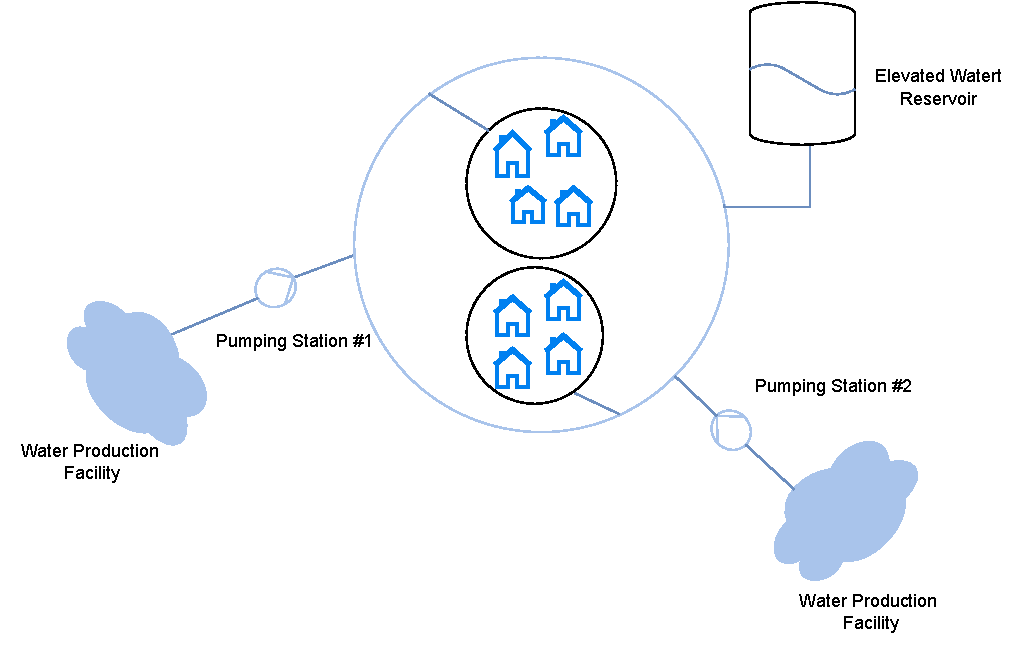
\includegraphics[width=0.6\linewidth]{Figures/WDNintro.pdf}
	\caption{A typical ring-type water distribution network with two pumping stations, multiple consumers and an elevated reservoir.}
	\label{fig:WDNintro}
\end{figure}

In order to verify the methods of this project are applicable in the real world, they are implemented on a water distribution network test setup.
  
\section{Test Setup}\label{sec:WDNsetup}
\cref{fig:WDN} presents the water distribution network test setup used in the project. The system consists of three parallel coupled pumps, acting as a pumping station which supplies water to a variable valve acting as a consumer zone, and an elevated water reservoir. For a comprehensive overview of component models in water distribution see \cite{Jensen}.

 \begin{figure}[h!]
	\centering
	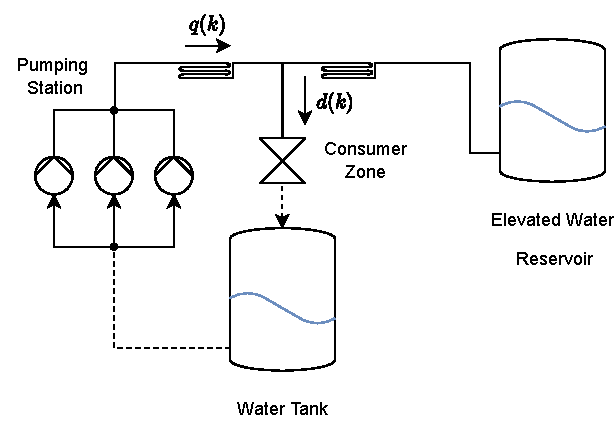
\includegraphics[width=0.81\linewidth]{Figures/WDN}
	\caption{Water distribution network with pumping station, consumer zone and elevated water reservoir.}
	\label{fig:WDN}
\end{figure}

The water tank is used to store water for the pumping station and is kept at a constant level with the help of a PI-controller that controls a set of auxiliary pumps.

The only dynamic component of the network seen in \cref{fig:WDN} is the elevated water reservoir, and can be described by the following differential equation:

\begin{equation}\label{eq:hDynamic}
	A\dot{h} = q + d \Leftrightarrow \dot{h} = \frac{q+d}{A}
\end{equation}  

\cref{eq:hDynamic} can be discretized by Euler's method:

\begin{equation}
	h(k+1) = h(k) + \frac{q(k)+d(k)}{A} 
\end{equation}

where,
\begin{center}
	\begin{tabular}{l p{10cm} l}
		$ h(k) $ & is the water level in the elevated water reservoir & [\si{m}]\\
		$ q(k) $ & is the flow of water through the pumps & [\si{m\cubed}/\si{s}]\\
		$ d(k) $ & is the water demand & [\si{m\cubed}/\si{s}]\\
		$ A $ & is the cross-sectional area of the elevated water reservoir & [\si{m\squared}]
	\end{tabular}
\end{center}

Note that the cross-sectional area of the elevated water reservoir is assumed constant along its vertical axis. \cite{Rathore930,MathiasJeppe730} uses the same elevated water reservoir as this project and states the following parameters:

\begin{table}[h!]
	\centering
	\begin{tabular}{|c|c|c|c|}
		\hline
		Diameter [\si{m}] & Height [\si{m}] & Cross sectional area [\si{m\squared}] & Capacity [\si{m\cubed}] \\ \hline
		0.6      & 0.706  & 0.283                & 0.2      \\ \hline
	\end{tabular}
	\caption{Elevated water reservoir parameters. Cross sectional is used in simulation.}
	\label{tab:Tank Parameters}
\end{table}

The power delivered to the water from the pumping station in \cref{fig:WDN} is:

\begin{equation}
			P(k) = q(k)\Delta{p}= q(k)(p_{out}(k)-p_{in}(k))
\end{equation}

Where the system pressure $ p_{out} $ is:

\begin{equation}
	p_{out}(k)=\rho g h_{ewr}(k)+\Delta{z}+\lambda_{1}\bigg(q(k)\bigg)+\lambda_{2}\bigg(q(k),d(k)\bigg)
\end{equation}

where,
\begin{center}
	\begin{tabular}{l p{10cm} l}
		$ \rho $ & is the density of water & [\si{l/m^{3}}]\\
		$ g $ & is the gravitational acceleration & [\si{m/s^{2}}]\\
		$\Delta{z}$ & is the drop in pressure due to geodesic level of tank & [\si{Pa}]\\
		$\lambda(\mathord{\cdot})$ & is the drop in pressure due to friction in a pipe-segment & [\si{Pa}] \\
		$p_{out},p_{in}$ & are the absolute pressure at outlet and inlet side of pumping station & [\si{Pa}]\\
	\end{tabular}
\end{center}

It is assumed that the pressure drop in the pipe connected to the pumping station, due to friction, takes the form: 

\begin{equation}
	\lambda_{1}\bigg(q(k)\bigg) = r_{1}\big|q(k)\big|q(k)
\end{equation}

and for a pipe connected to an elevated water reservoir the pressure drop takes the form: 

\begin{equation}
	\lambda_{2}\bigg(q(k),d(k)\bigg) = r_{2}\big|q(k)-d(k)\big|\bigg(q(k)-d(k)\bigg) 
\end{equation}

with friction constants $ r_{i} $.

The pump inlet is assumed open to atmosphere and the inlet pressure becomes $p_{in} = 0$. The power delivered from the pumping station is:

\begin{equation}\label{eq:WDN_Power}
P(k)= q(k)\bigg(\rho g h_{ewr}(k)+\Delta{z}+\lambda_{1}\bigg(q(k)\bigg)+\lambda_{2}\bigg(q(k),d(k)\bigg) \bigg) 
\end{equation}
 
\section{Consumption Model}\label{sec:Consumption}
Real water consumption data is analysed. A historical dataset of daily water consumption over a three months period has been provided by Grundfos, which contains data sampled four times per hour. \cref{fig:Consumption} depicts consumption of a 24 hour period. Note that the unit of the consumption data is unknown and that \cref{fig:Consumption} is normalised. 

\begin{figure}[h!]
	\centering
	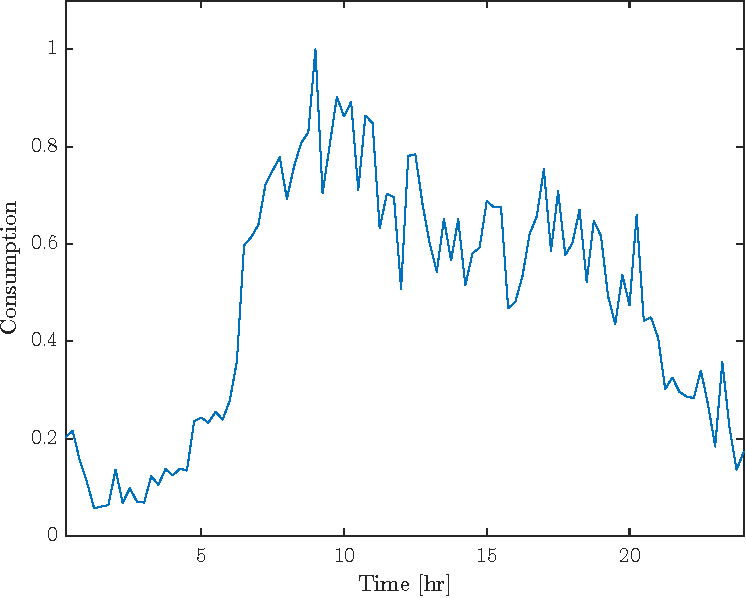
\includegraphics[width=0.7\linewidth]{Figures/Consumption.pdf}
	\caption{Consumption profile in a day.}
	\label{fig:Consumption}
\end{figure}

The power equation presented in \cref{eq:WDN_Power} will in the following section be used to select states and action of the system, such that reinforcement learning can be used as a control method. The consumer data will be used to emulate the consumption of a consumer zone, and will play a role when doing full state function approximation Q-learning.

\newpage